\begin{artengenv}{Jerzy Dajka}
	{Past of a quantum particle: old problem with recent controversies}
	{Past of a quantum particle: old problem with recent controversies}
	{Past of a quantum particle: old problem with recent controversies}
	{University of Silesia in Katowice}
	{Time-symmetric formulation of quantum mechanics---the two-state vector formalism---is presented  as a tool for studying past behaviour of quantum systems. A role of weak measurement and weak values in the Cheshire Cat effect and a nested (Vaidman) three-path interferometer are discussed. Interpretation of particle's faint trace indicating possibility of discontinuous  paths of particles passing  the Vaidman interferometer is given.   Consistent histories are presented as one of  alternative approaches.  Multitude of controversial issues is briefly reviewed and discussed. }
	{two-state vector formalism, weak values, weak measurement, Cheshire Cat effect}



\section{Introduction}
\lettrine[loversize=0.13,lines=2,lraise=-0.01,nindent=0em,findent=0.2pt]%
{C}{}openhagen orthodoxy limits predictive role of quantum mechanics to measurement results only and introduces unavoidable indeterminacy at a quantum level. One can prepare (preselect) a quantum system, evolve it (via e.g. unitary time evolution) and then one can measure it and postselect a particular, desired result. The measurement output is known to belong to a certain and well defined set of possible values which occur, as an output, with certain probability. Such an approach is already more than century old and we are used to an uncomfortable fact that at a  quantum level not only measurement result but also quantum measurement {\it per se} requires an interpretation. 

In a  standard von Neumman's scheme a measurement output of an observable   is one of eigenvalues $a_k$ of  a hermitian operator $A$ representing the observable i.e. $A|a_k\rangle=a_k|a_k\rangle$ with the corresponding eigenvectors  $|a_k\rangle$ forming a basis spanning a state space of the system. Let us forewarn that for a simple convenience we use notation suitable for qudits (finite $d$--dimensional quantum systems) rather than general quantum systems. Such a convention allows one to bound an applied formalism almost solely to linear algebra at a low cost of a little  mathematical 'flexibility' required for studying infinite systems.  Having a system in a state $|\psi\rangle=\sum_k c_k |a_k\rangle$ a probability of measuring $a_k$ is given by a scalar product of the state and the particular eigenstate  $|a_k\rangle$ and reads  $prob(k)=|\langle a_k|\psi\rangle|^2$. We humbly acknowledge that one cannot say {\it before} the measurement is done which among $a_k$'s is going to be  observed and we are left with an expectation only:   $\langle A\rangle =\langle\psi| A|\psi\rangle=\sum_k p_k a_k$. Moreover, we know that such a measurement procedure
     causes a  serious disturbance of a system as it results in  a jump or collapse of the state $|\psi\rangle\rightarrow|a_k\rangle$ which can be formalised in terms of projection operators $|a_k\rangle\langle a_k|$. 



In more formal terms, with an applied notation summarized in Tab.(\ref{tabx}), one prepares a composite state of a system and a probe (a pointer) 
  $|\Psi(t_i)\rangle=|\psi(t_i)\rangle|\phi(t_i)\rangle$. 
  %
\begin{table}[ht]
\centering
\begin{tabular}{|l||l|}
\hline
states of  &applied  notation \\
\hline
\hline
system+probe & $|\Psi\rangle$ (capital)\\
%\hline
system preselected& $|\psi\rangle$, $|a\rangle$ \\
system postselected& $|b\rangle$ \\
%\hline
probe only& $|\phi\rangle$\\
\hline

\end{tabular}
\caption{\label{tabx} Notation of states applied in the paper with time parameter and subscripts skipped.}
\end{table}
  To measure a system, the probe must, at least for a certain duration $\tau$, interact with the measured object. Measuring an observable $A$ one assumes that the system--probe interaction is given by a Hamiltonian coupling $A$ and a 'momentum' (an operator canonically conjugated to the  probe position) 
  \mbox{$H_{int}=g(t)AP$} with a coupling strength $g=\int_{t_i}^{t_i+\tau} g(t)dt$. 
  Hence, the von Neumann ideal measurement is nothing but a dynamic process 
     \begin{equation}\label{ideal}
    |\Psi(t_i+\tau)\rangle=e^{-igAP}|\psi(t_i)\rangle|\phi_{x_0}\rangle=
        \sum_k|a_k\rangle\langle a_k|\psi(t_i)\rangle e^{-iga_k P}|\phi_{x_0}\rangle=\sum_k|a_k\rangle\langle a_k|\psi(t_i)\rangle|\phi_{x_0-ga_k}\rangle \end{equation}
causing shift of a pointer position from $x_0$ (in the state $|\psi_{x_0}\rangle$ to $x_0-ga_k$ for $|\phi_{x_0-ga_k}\rangle$. The last step, i.e. a projective measurement of the pointer, allows one to relate a particular  read-out value $x_0-ga_k$ to a particular value $a_k$ of the observable $A$. 

It is not surprising that there are circumstances where  limitations of Copenhagen interpretation (and the celebrated eigenvalue--eigenstate link) become quite bothersome. We present here only one of many problems: 
a measurement result allows to gain knowledge about the present of quantum systems (a particle). It is, however, hardly possible to infer upon that what was the particle's {\it past}, what 'historic' properties one can attribute to the just measured systems. Sometimes  it is even harder to say anything about  quantum systems which are essentially closed (as, for example, the whole universe is) and do not allow to include an external observer keeping a pointer or these which are simply resistant to measuring attempts. Neutrino, hardly interacting with anything, can serve as a natural example of such a 'measurement--resistive' system. Counterfactual reasoning  (what would happen if a particular measurement were performed  or, more generally,  if there were that $a$, then it would be that $b$) is related to an another branch of problems where the eigenvalue--eigenstate link induces unwanted constraints. 

Our aim is to present a seemingly simple quantum system -- a particle in a nested three-path interferometer invited by Lev Vaidman to a modern scientific debate. A particle enters the interferomenter, it has three paths at its disposal and then it is measured (postselected) leaving the inteferometer by one of three exits. The question which is asked looks innocent and apparently simple: what path took the particle inside the inteferometer? What was its trajectory? The questions are natural (particles entering and leaving the inteferometer must somehow pass it) and interesting (cf. reference list below) although  from the Copenhagen prospective slightly out of place.  In this paper we focus on  the two-state vector formalism recently applied to answer the above question and leading to hardly acceptable and very disputable possibility: the particle in the Vaidman interferometer follows {\it discontinuous}  path. Surprisingly, such a weird answer, seemingly contradicting not only our intuition but also common sense,  is supported by very recent experiments and as such requires careful analysis not only from physical but also more fundamental, philosophical perspective. Although the two-state vector formalism is nothing but a time-symmetric version of a very standard quantum mechanics, it exhibits its true predictive power combined with a notion of {\it weak measurement} and {\it weak value} of an observable. Both concepts, exemplified with help of the Cheshire Cat effect, are lacking from the eigenvalue-eigenstate link and require an interpretation.  The paper is organized as follows: in Sec. 2 the two-state vector formalism is presented, a notion of weak measurement and weak values are applied to present the Cheshire Cat effect of a spatial separation of a photon position and polarization. Sec 3. is devoted to the Vaidman's construction of a nested  interferometer and a faint trace  as a tool verifying a presence of a weakly measured particle inside the interferometer. As  the two-state formalism is not the only formalism applied to study particle's past in the Vaidman interferometer,    in Sec 4. we very briefly present one of  alternatives: an approach based on consistent histories and we indicate probably the  most obvious and easiest to formulate objection against this approach. Concluding in Sec 5. we list selected problems which---at least in our opinion---urgently require a professional philosophical analysis. 

\section{Two--state vector formalism and the Cheshire Cat}

Classical dynamics of a particle is a solution of the Newton equation which, to predict uniquely a final state, needs initial conditions (an initial state) to be specified. For quantum system to predict a measurement output at a given time it is not enough to preselect an initial state and then to solve the Schr\"{o}dinger equation as a resulting final state may be a superposition. To get unique prediction of a measurement output one needs an additional information what state was postselected at the end of evolution.  In other words, in classical physics all the results of future measurements are constrained by the results of the past measurements leading to an initial preparation. For quantum systems, however, a measurement output is only partially determined by past measurements and we recognize that quantum mechanics, contrary to the classical one, is essentially time asymmetric. This asymmetry limits an ability of reproducing the  past solely upon the present measurement results. The two-state vector formalism~\parencite{Aharonov2008} (TSVF) is an attempt to make quantum mechanics time-symmetric by adding an information concerning a postselected state. According to the TSVF, to describe a quantum system at a time $t$ one needs a two-state vector
\begin{equation}\label{tsv}
    \langle \omega(t)|\,\,|\alpha(t)\rangle
\end{equation}
where $|\alpha(t)\rangle$ is a 'usual' state of a time-evolving quantum system which is a fundamental object of a standard quantum mechanics and $\langle\omega(t)|$ is a state evolving {\it backward in time} and  determined by the results of measurements performed on the system {\it after} the time $t$. In other words, the two-state vector is pair of states consisting of   a forward evolving preselected state  and a backward evolving postselected state. 
Let us imagine that at $t=t_i$ our system is in one of eigenstates of an observable $A$ i.e. $|\alpha(t_i)\rangle=|A=a\rangle$ and finally, at $t=t_f$, $\omega(t_f)\rangle=|B=b\rangle$ for a different observable $B$. According to the TSVF a complete information about the system at $t\in(t_i,t_f)$ is encoded in $\langle \omega(t)|\,\,|\alpha(t)\rangle$ where
\begin{equation}
   \begin{split}
       |\alpha(t)\rangle = U(t,t_i)|A=a\rangle\\
       |\omega(t)\rangle= U(t,t_f)|B=b\rangle
   \end{split}
\end{equation}
and $U(\cdot,\cdot)$ is a unitary time evolution operator. 
Let us strongly emphasise that essentially the TSVF is a standard quantum mechanics just equipped with an additional information carried by a backward evolving state. As such, the TSVF is not expected to contradict any 'standard' predictions of the quantum mechanics.  Minimalists may consider TSVF just as a useful tool to analyze otherwise strange and 'paradoxical' phenomena.   


Let us describe the following scenario to present a rationale behind the TSVF construction and to show a particular usefulness of this formalism in a weak measurement context. 
The Aharonov-Bergmann-Lebowitz rule~\parencite{abl} is a working horse of many of subsequent techniques. If there is a quantum system preselected in a state $|\psi(t_i)\rangle$ and finally found in  a postselected state $|b_f\rangle$ conditioned probability that an observable $A=\sum_n a_n|a_n\rangle\langle a_n|$ measured at some intermediate stage gives $a_n$ reads as follows:
\begin{equation}\label{abl}
    prob(a_n)=\frac{|\langle b_f|a_n\rangle\langle a_n|\psi(t_i)\rangle|}{\sum_s|\langle b_f|a_s\rangle\langle a_s|\psi(t_i)\rangle|^2}.
\end{equation}
We consider a narrow time window $t_w\pm\tau/2$ when the pointer--system interaction takes place. Out of this window a time evolution of a system+probe composite is unitary and governed by $U$. Then, a time evolved system--pointer state reads as follows: 
\begin{equation}
\begin{split}
    |\Psi(t)\rangle= U(t,t_w) e^{-gAP} U(t_w,t_i) |\psi(t_i)\rangle|\phi(t_1)\rangle=U(t,t_w) e^{-igAP}|\psi(t_w)\rangle|\phi(t_1)\rangle\\
=U(t,t_w)\sum_k e^{-iga_kP}\langle a_k|\psi(t_w)\rangle |a_k\rangle |\phi(t_i)\rangle
\end{split}
\end{equation}
Finally, at $t=t_f$, the system becomes postselected i.e. it is subjected to an (ideal) projective measurement of an observable $B$ reducing its state to of eigenstates $|b_f(t_f)\rangle$ of $B$. Upon the Aharonov-Bergmann-Lebowitz rule the pointer after the system postselection is left in  a state
\begin{equation}
|\phi(t_f)=\sum_k[\langle b_f(t_f)|U(t_f,t_w)|a_k\rangle\langle a_k|\psi(t_w)\rangle]e^{-iga_kP}|\phi(t_i)\rangle      
\end{equation}
Let us note that, at least formally, $\langle b_f(t_w)|=\langle b_f(t_f)|U(t_f,t_w)$ is a bra-vector which is dual to a state  
$|b_f(t_w)\rangle=[\langle b_f(t_w)]^\dagger=[\langle b_f(t_f)|U(t_f,t_w)]^\dagger=U^\dagger(t_f,t_w)|b_f(t_f)\rangle=U(t_w,t_f)|b_f(t_f)\rangle$
which, in turn, is a postselected system state  
evolving {\it backward} in time.
 If in addition  the system-probe interaction is weak---i.e. $g\ll 1$---one can expand $e^{-iga_kP}\approx 1-iga_k P$ and obtain
\begin{equation}
    |\phi(t_f)\rangle=\langle b_f(t_w)|\psi(t_w)\rangle \left( 1-ig\langle A\rangle^w P\right)|\phi(t_i)\rangle=\langle b_f(t_w)|\psi(t_w)\rangle\exp(-ig\langle A\rangle^wP)|\phi(t_i)\rangle
\end{equation}
where the quantity
\begin{equation}\label{weak}
    \langle A\rangle^w=\frac{\langle b_f(t_w)|A|\psi(t_w)\rangle}{\langle b_f(t_w)|\psi(t_w)\rangle}
\end{equation}
 defines a {\it weak value}~\parencite{primus} of $A$. The weak value is thus a number characterizing
a shift (or a motion) of a quantum pointer due to a weak interaction with a measured system. Although the weak value is generically  complex, it is a measurable quantity~\parencite{weak_rmp} and its real part can be interpreted as an amplitude of a measurement induced transition from a preselected into postselected state. Its squared modulus gives the corresponding probability of the process. Such an interpretation settles  weak values in a natural context of a measurement driven dynamic process. 

Quantum weak values~\parencite{primus} attract non--decreasing attention of physicists who  apply them to analyze otherwise difficult problems. Let us mention only two examples: continuous and sometimes controversial discussion what the history of quantum particle really is~\parencite{PhysRevA.87.052104,PhysRevA.89.024102,PhysRevA.96.022126} or one of the  spectacular counter-intuitive effects---the quantum Cheshire Cat~\parencite{cat}. Weak values seem to be of a particular usefulness in all the circumstances which  require simultaneous measurement of otherwise non co--measurable observables~\parencite{cat,weak,e20110854,Aharonov2008,weak_rmp}.  
%
Let us emphasise one but crucial feature concerning {\it null} weak values. In a well established scheme of an ideal measurement Eq.(\ref{ideal}) the pointer state couples to a particular eigenvector with a particular eigenvalue $a_k$. If $a_k=0$ there is no effect on a pointer state and the probe remains not 'shifted'. There is however an obvious modification of the system state which is projected on a subspace corresponding to the null eigenvalue. In the weak measurement scheme situation essentially differs. If a particular {\it weak value} vanishes $\langle A\rangle^w=0$  and a postselected state of a system is obtained  the property corresponding to $A$ cannot be detected. The weak value indicates a
coupling-induced imprint which is left on the pointer, conditioned on the postselection. As a  consequence, the vanishing weak value
correlates successful postselection with the quantum pointer having been left unchanged despite the interaction with the system. Let us emphasise that for  weak values Eq.(\ref{weak})  there is no clear analogy of the eigenvalue-eigenstate link and their relation to quantum properties remain a subject of an intensive investigation~\parencite{Matzkin_prop,weak,e20110854} 

To explore further an interpretation of null weak value (further used in a general context of a past of quantum particles ~\parencite{PhysRevA.95.032110,PhysRevA.97.046102,PhysRevA.97.046103}) we discuss one of the first quantum phenomena exhibiting non--intuitive predictions based upon weak values and weak measurement scheme: the Cheshire Cat effect~\parencite{cat,cat_schlos}. For the sake of making our discussion as self--contained as possible we recall a very basic idea of the  Cheshire Cat as primarily introduced in Ref.~\parencite{cat}.   The quantum Cheshire Cat effect~\parencite{cat} indicates  separation of internal and external degrees freedom of a quantum system corresponding to the Cat's position and the grin respectively and justifying a direct implementation of terminology adopted from Carroll's novel {\it Alice’s Adventures in Wonderland}. 
%
The archetype of the Cheshire Cat~\parencite{cat} is a photonic system and an effect takes place in a {\it two--path} Mach-Zehnder setting with a
path 'chosen' by  the photon---either left $L$ or right $R$---describing the 'external' degree of freedom  and photonic polarization---horizontal $\leftrightarrow$ or vertical $\updownarrow$ representing internal degree of freedom as it is presented in Fig.(\ref{cat}) or on Figure 1 of Ref.~\parencite{cat}. 
\begin{figure}
 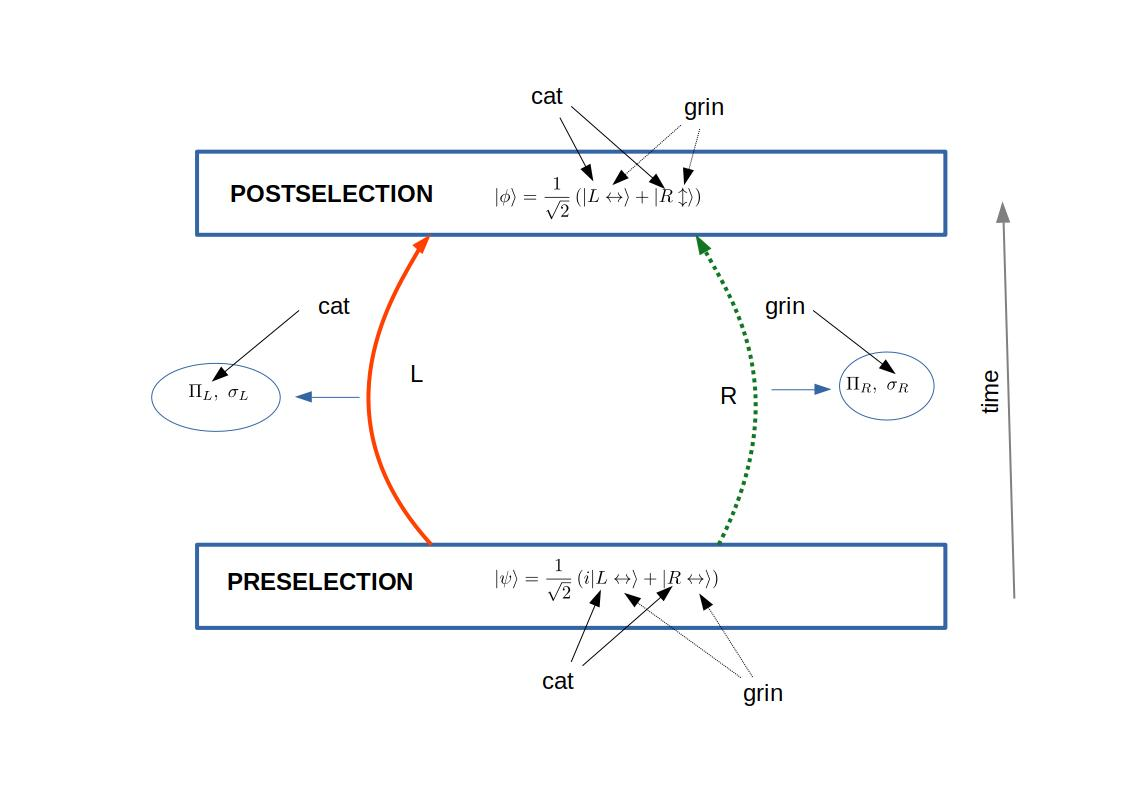
\includegraphics[width=1.0\textwidth]{ART_dajka/cat.jpg}%
 \caption{The Cheshire Cat effect. Photon in an interferometer is preselected in a state $|\psi\rangle$.  It is then  {\it weakly} measured along left and right arms (possible $L,R$ paths)  and then postselected in a state $\phi\rangle$. The weak values $
\langle \Pi_L\rangle^w =1$,
$\langle \Pi_R\rangle^w=0$, 
$\langle \sigma_L\rangle^w =0$ and $\langle \sigma_R\rangle^w=1$ interpreted as a presence of the Cat in the left arm and its grin in the right one indicate separation of photon polarization ('grin') and photon position. }\label{cat}
\end{figure}
Effectively, both types of degree of freedom are qubits i.e. a state space of the  system is
$\mathcal{H}=\mathbf{C}^2\otimes\mathbf{C}^2=\mbox{span}\{|L\rangle,|R\rangle\}\otimes\mbox{span}\{|\leftrightarrow\rangle,|\updownarrow\rangle\}$  
where $L,R$ and $\leftrightarrow,\updownarrow$ label the 'external' and internal degrees of freedom respectively. 
Detection of  the Cat's position  corresponds to a measurement related to the projectors: $\Pi_L=|L\rangle\langle L|$ and $
\Pi_R=|R\rangle\langle R|$
whereas a measurement of Cat's grin (an internal degree of freedom) in a given (either left or right) position requires the projectors $\sigma_L = \Pi_L \sigma_z$ and $\sigma_R =  \Pi_R \sigma_z$
where  $\sigma_z=|+\rangle\langle+|-|-\rangle\langle -|$ for $|\pm\rangle=[|\leftrightarrow\rangle \pm i|\updownarrow\rangle]/\sqrt{2}$. 
%
According to the proposal given in~\parencite{cat}, the system is preselected (prepared) in a  specific but not entangled state
$|\psi\rangle = \frac{1}{\sqrt{2}}\left(i|L\leftrightarrow\rangle +|R \leftrightarrow\rangle\right)$
and, after passing the interferometer,  postselected in a state
$|\phi\rangle = \frac{1}{\sqrt{2}}\left( |L\leftrightarrow\rangle +|R \updownarrow\rangle\right)$.   
%
In the meantime, one measures {\it weak values} Eq.(\ref{weak}) of the quantities $\Pi_{L,R}$ and $\sigma_{L,R}$ i.e. weak values of the Cat's position and grin respectively. One obtains~\parencite{cat}
$
\langle \Pi_L\rangle^w =1$,
$\langle \Pi_R\rangle^w=0$, 
$\langle \sigma_L\rangle^w =0$ and $\langle \sigma_R\rangle^w=1$. 
% 
Whenever a weak value is null the corresponding quantum property (either the Cat's presence or its grin in one of two arm of the interferometer) is absent in a particular arm  where the weak measurement was performed. With such an interpretation we infer that a presence of the Cat (indicated by $
\langle \Pi_L\rangle^w \neq 0$) in the left $L$ arm of the interferometer is accompanied by a presence of Cat's grin in the right $R$ interferometer's arm as indicates $\langle \sigma_R\rangle^w\neq 0$. Clearly, the description provided here is far from being complete. In particular it does not take into account specific experimental circumstances typical for realistic Cheshire Cat measurements~\parencite{dup}, recent experiments~\parencite{c2,cat_schlos} or an effect of decoherence~\parencite{schloss} modyfying weak values~\parencite{Shik} and the Cheshire Cat predictions~\parencite{mojkot,mojkot1}. Moreover, interpreting null weak value as a hallmark of a '{\it non-presence} of something' is controversial and  far from being commonly accepted  
~\parencite{PhysRevA.95.032110,PhysRevA.97.046102,PhysRevA.97.046103,vaid_trans,lady}. 
\begin{figure}
 \includegraphics[width=0.8\textwidth]{ART_dajka/vaid1a.eps}\\%
 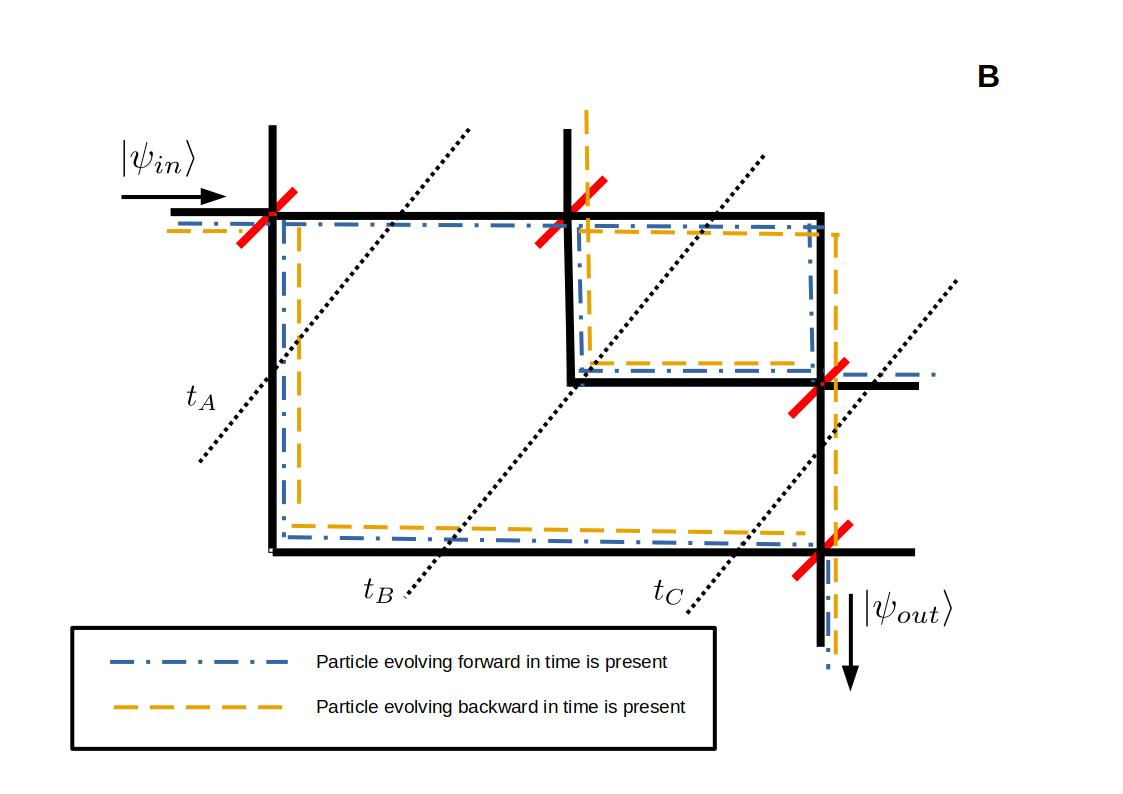
\includegraphics[width=0.8\textwidth]{ART_dajka/vaid1b.jpg}%
 \caption{Vaidman  interferometer consisting of four beam splitters $BS_{1,2,3,4}$ acting as unitary transformation in Eq.(\ref{bs}). In  {\it panel A} there are  three 'paths' Eq.(\ref{baz}) indicted  $I,II,III$ and labelled by different colours. An entrance of an input a particle in a state $|\psi_{in}\rangle$ and an exit of a particle in a state $|\psi_{out}\rangle$ are indicated by arrows. Time instants  $t_{A,B,C}$ when  weak measurements take place are indicated by dotted lines in  {\it panel B}. The dash-dot and dash lines shown in a legend box of {\it panel B} indicate  a {\it non-zero} amplitude for meeting a particle evolving forward and (respectively) backward in time. According to the TSVF the particle leaves a faint trace only if {\it both lines} coincide i.e. on a green path ($III$) and inside the internal interferometer as it is indicated in {\it panel B}.}\label{fig0}
\end{figure}

\section{Faint trace of a particle in a Vaidman interferometer}



Quantum particle can be prepared (preselected) in a given and desired state and may also be postselected in another state with a known at least in principle probability. That what occurs in between, what is the particle's past, remains problematic due to specific features of quantum measurements, cf. Eq.(\ref{ideal}), unavoidably modifying quantum states of measured objects. It is particularly important if one asks about a history of a quantum particle passing trough interferometer: the particle enters the device and leaves it (if its outcome is measured), however, inside the interferometer, unless it's coherence is lost, the particle leaves nothing but a faint trace {\it defining} its presence, a faint trace which
is a result of a {\it small} change of an amplitude of a component orthogonal to an undisturbed particle's state (weakly). Such a faint trace is measurable  only in experiments operating on an
ensemble of particles having the same pre-- and postselection.
%
%
Past of a quantum particle in a nested Mach--Zehnder interferometer ({\it Vaidman interferometer})-- proposed~\parencite{PhysRevA.87.052104} and presented in Fig.(\ref{fig0})  -- was recently studied in Ref.~\parencite{PhysRevA.87.052104} using 
quantum weak values~\parencite{primus,weak,Aharonov2008} and the two state vector formalism (TSVF)~\parencite{Aharonov2008}. In this approach the faint trace is left by a particle unless a {\it weak value} of an appropriate projecting operator vanishes. A weak measurement of particle traces, contrary to a traditional and collapse assisted one, hardly perturbs the system maintaining its coherence sufficiently for interference effects to occur. The results, however, are highly confounding:  particles seem to follow anomalous {\it discontinuous} path. Such a seemingly weird conclusion results in plethora of controversies~\parencite{PhysRevA.88.046102,PhysRevA.88.046103}, some of them are quite recent cf. Ref.~\parencite{lady}, and since that time  (almost) all  works  on that problem  have came in triads: a paper, commentary inspired by the paper and a reply to the comment~\parencite{PhysRevA.88.046102,PhysRevA.88.046103}.  
The main reason is that the TSVF~\parencite{Aharonov2008} applied in Ref.~\parencite{PhysRevA.87.052104} is one of few possible approaches to investigate quantum past. The other non--equivalent alternatives are consistent (decoherent) histories~\parencite{PhysRevA.94.032115,PhysRevA.95.066101} (briefly presented below), standard quantum mechanics~\parencite{PhysRevA.96.022126,PhysRevA.99.026103,PhysRevA.99.026104} and many other other alternative studies
~\parencite{PhysRevA.91.012103,PhysRevA.93.036103,PhysRevA.92.023829,PhysRevA.93.017801, Hashmi_2016,Vaidman_2018,Hashmi_2018,elitzur}. Moreover, even recent experiments and their detailed analyses fail to resolve all the controversial issues~\parencite{PhysRevLett.111.240402,10.3389/fphy.2015.00047,10.3389/fphy.2015.00048,Sponar_2019,PhysRevA.95.042121,PhysRevA.97.052111, PhysRevA.97.052111,PhysRevA.89.033825,elitzur,WIESNIAK20182565}.  
A conception of
discontinuous path is clearly counter--intuitive but there are analyses~\parencite{e20110854,PhysRevA.101.052119} and claims which support the faint--trace anomalous picture as experimentally confirmed.  


For a sake of completeness we formalize the Vaidman interferometer and review the controversial features of the faint traces of particles passing it. The original Vaidman interferometer is presented in Fig.(\ref{fig0}). It consists of spatial degree of freedom given by three paths denoted by $\RN{1},\RN{2},\RN{3}$ respectively and four beam splitters. The Vaidman interferometer can effectively be described~\parencite{PhysRevA.96.022126,PhysRevA.99.026103,PhysRevA.99.026104,scirep} as a three level quantum system (a qutrit) with a state space spanned by an orthonormal basis
%
\begin{equation}\label{baz1}
|\RN{1}\rangle=\left(\begin{array}{c} 1 \\ 0 \\ 0   
\end{array}\right),\,\,|\RN{2}\rangle=\left(\begin{array}{c} 0 \\ 1 \\ 0   
\end{array}\right)  \mbox{and}\,\,\,\, |\RN{3}\rangle=\left(\begin{array}{c} 0 \\ 0 \\ 1   
\end{array}\right)
\end{equation}
%
Let us note an intuitively acceptable rationale behind imposing orthogonality on the set Eq.(\ref{baz1}): if a particle collapses to a particular state in Eq.(\ref{baz1}), at the same time there is no amplitude to be in an another one.  
%
In an ideal setting of a noise--less system (for a noisy dephasing model cf. Ref.~\parencite{scirep}), a passage of a particle is described by a unitary transformation composed of four unitaries $U_4U_3U_2U_1$ corresponding to subsequent beam splitters termed as $BS_{i}, i=1, \ldots, 4$ in Fig(\ref{fig0}):
\begin{equation}\label{bs}
U_1 = U_4 =\frac{1}{\sqrt{3}}\left( \begin{array}{ccc} \sqrt{3} & 0 & 0 \\ 0 & -1 & \sqrt{2} \\ 0 & \sqrt{2} & 1  
\end{array}\right)\,\,  \mbox{and}\,\,\,\,
U_2 = U_3 =\frac{1}{\sqrt{2}}\left( \begin{array}{ccc} 1 & 1 & 0 \\ -1 & 1 & 0 \\ 0 & 0 & \sqrt{2}  
\end{array}\right)
\end{equation}
The strategy applied  in Ref.~\parencite{PhysRevA.87.052104} to infer the path of a particle entering  and leaving Vaidman interferometer  in a state $|\RN{3}\rangle$  was to investigate its {\it weak trace}  at three instants $t_A,t_B,t_C$ indicated in Fig.(\ref{fig0}). In a framework of the TSVF~\parencite{Aharonov2008} and according to Ref.~\parencite{PhysRevA.87.052104} the weak trace is indicated by  a non--vanishing weak value~\parencite{primus,PhysRevA.95.032110} of one of the  projectors
%
\begin{eqnarray}\label{weak0}
\langle\Pi_i\rangle_w^q&=&\frac{\langle\psi_{post}^q|\Pi_i|\psi_{pre}^q\rangle}{\langle \psi_{post}^q|\psi_{pre}^q\rangle}, \,\,\,  \mbox{where}\,\,\,\,\Pi_i =  |i\rangle\langle i|,\,\, i=\RN{1},\RN{2},\RN{3}  \,\,\,  \mbox{and} \,\,\, q=A,B,C  
\end{eqnarray}
where forward in time evolving preselected state (directly prior to the measurement of $\Pi_i$) and backward in time postselected state (immediately after the measurement) states compose  a {\it two--state vector} $\langle\psi_{post}||\psi_{pre}\rangle$. 

Most of controversies originate from highly counter--intuitive conclusions provided in Ref.\parencite{PhysRevA.87.052104} indicating possibility of discontinuous trajectories followed by a particle passing trough Vaidman interferometer. There are three instants $t_A,t_B,t_C$ where the weak trace is measured: $A$: just after it passes the interferometer  $BS_1$ but before it arrives to $BS_2$, $B$: where the weak measurement becomes conducted for all three potential paths and $C$: after the $BS_3$ beam splitter as presented in Fig.(\ref{fig0}). The corresponding  forward-in-time evolving preselected states read as:   
$
|\psi_{pre}^A\rangle = U_1|\RN{3}\rangle$, $
|\psi_{pre}^B\rangle = U_2U_1|\RN{3}\rangle$ and $|\psi_{pre}^C\rangle = U_3U_2U_1|\RN{3}\rangle$. 
In the time--symmetric TSVF setting the  postselected states 
$|\psi_{post}^A\rangle = U^\dagger_2U^\dagger_3U^\dagger_4|\RN{3}\rangle$, $|\psi_{post}^B\rangle =U^\dagger_3U^\dagger_4|\RN{3}\rangle$ and $|\psi_{post}^C\rangle =U^\dagger_4|\RN{3}\rangle$ describe a hypothetical particle detected at $\RN{3}$ evolving backward in time. Results of the weak measurement are summarized in Tab.(\ref{tab0}). 
%
\begin{table}[ht]
\centering
\begin{tabular}{|l||lll|ll|}
\hline
$\langle\Pi_{\RN{1},\RN{2},\RN{3}}\rangle_w^{A,B,C}$ & $\RN{1}$ & $\RN{2}$ & $\RN{3}$ &$U_{pre}^{A,B,C}$ & $U_{post}^{A,B,C}$ \\
\hline
\hline
A & 0 & 0 & 1 & $U_1$ & $U^\dagger_2U^\dagger_3U^\dagger_4$\\
%\hline
B & -1 & 1 & 1 & $U_2U_1$ & $U^\dagger_3U^\dagger_4$ \\
%\hline
C &  0 & 0 & 1 & $U_3U_2U_1$ & $U^\dagger_4$\\
\hline

\end{tabular}
\caption{\label{tab0} Weak traces $\langle\Pi_{\RN{1},\RN{2},\RN{3}}\rangle_w^{A,B,C}$ Eq.(\ref{weak0}) of a particle in Vaidman interferometer in Fig.(\ref{fig0}) at different instants $A,B,C$ indicated in Fig.(\ref{fig0}) and corresponding pre-- and postselections given by $|\psi_{pre}^{A,B,C}\rangle=U_{pre}^{A,B,C}|\RN{3}\rangle$ and $|\psi_{post}^{A,B,C}\rangle=U_{post}^{A,B,C}|\RN{3}\rangle$ respectively. It follows that at $t_A$ and $t_C$ a particle leaves its weak trace on paths $\RN{1}$ and $\RN{3}$ respectively whereas at $t_B$ a faint trace is present on each of three paths.}
\end{table}
According to Ref.~\parencite{PhysRevA.87.052104} a presence of a particle is defined by 
its non--vanishing weak trace. The counter--intuitive conclusion which can be inferred upon the results summarized in Tab.(\ref{tab0}) is the following: at $A$ and $C$ the particle is present in $\RN{3}$, what upon Fig.(\ref{fig0}) is intuitively acceptable, but at $B$ it is also present in an internal loop ($\RN{1},\RN{2}$) of the Vaidman interferometer.  The above formal analysis one can support  utilizing the TSVF and a {\it sine qua non} condition for a presence of particle: to get a non-vanishing  
{\it weak value} of a  particular projector in a  weak measurement scheme  both the amplitudes of  forward and backward evolving component of the two--vector  necessarily   must  not vanish.  The regions where the amplitudes of forward and backward evolving states do not vanish are depicted in Fig.(\ref{fig0}) with dash-dot and dash lines respectively. The only regions where the lines coincide are the path labeled by $\RN{3}$ and the internal loop of the Vaidman interferometer. There is a faint trace left by  particles  on the path $\RN{2}$ neither between beam splitters $BS_1$ and $BS_2$ (potentially used  photons entering the internal loop) nor between $BS_3$ and $BS_4$ where the photons could exit the internal loop. In simple words, upon the TSVF we conclude that a presence of a particle indicated by a faint trace  in an internal loop is not accompanied by any trace of a particle entering or leaving the internal loop and the particle path is 
{\it discontinuous}.  It is obvious that such a confounding result needs further experimental verification. One can safely assume that any potential experiment, as it was so far, will be highly subtle and sophisticated~\parencite{e20110854,PhysRevA.101.052119,pnas,pnas1}. 







%\section{Cheshire cats and conterfactual communication}

\section{Consistent histories as an alternative}  

Orthodox (Copenhagen orthodox) researchers claim that one 
cannot talk about a quantum particle between measurements at all. This is an obvious limitation of standard quantum theory radically excluding important questions related to a past behaviour of quantum systems.   
%
Previously discussed  two--state vector formalism~\parencite{Aharonov2008} and consistent (or decoherent) histories approach~\parencite{Griffiths,Griffiths1984,Omnes1988,Omnes1,gel1,gel} serve  as fruitful examples of theoretical extensions  going beyond (and sometimes across) the Copenhagen interpretation. In particular,  we have recently been  witnessing how  the two above mentioned approaches are competitively applied to a  problem  of a past behaviour of a quantum particle in a Vaidman interferometer~\parencite{PhysRevA.87.052104,PhysRevA.95.066101,scirep}. Using different methods, consistent histories allow one to gain an additional insight if they are applied to  problems  ranging from a small but fundamental~\parencite{GRIFFITHS_measur,GRIFFITHS_onto,Griffiths2014,mea1} to the largest scale~\parencite{zur1,q_cosm}. The consistency of  histories  allows one
to assign probabilities to sequences of suitably defined events for a quantum system. As the quantum events in this perspective  do  not rely on the notion of measurement {\it per se}, the consistent histories approach enables one to design a new type of logical approach~\parencite{Griffiths1984} which is essentially different to the Birkhoff and von Neumann quantum logic~\parencite{qlog}. There is a particular practical advantage of using consistent histories formalism to gain information about a system if
an external measurement is not available either because of fundamental or simply technical reasons as it is in the case of  Vaidman interferometer where an experiment output is highly sensitive to a measurement-induced coherence deficiency. 
%
Quantum reasoning based on consistent histories~\parencite{Griffiths_reason} uses projective decomposition of identity $PDI=\{P^k\}$ 
where $P^jP^k =\delta_{jk}P^k$ and $\sum_j P^j=I$
as its cornerstone~\parencite{Griffiths}. It   serves as a quantum-mechanical counterpart of an event algebra used in a standard stochastics. There is, however, one  crucial yet fundamental requirement which is additionally imposed: {\it the single framework rule}~\parencite{Griffiths,Griffiths_reason,GRIFFITHS_measur}. According to that rule  simultaneous reasoning to physical properties is meaningful if it is limited to  'events'  which are compatible~\parencite{Griffiths,Griffiths_reason,GRIFFITHS_measur,GRIFFITHS_onto}. 
At each time instant all  quantum properties of a system correspond to elements of an instantaneous PDI having assigned probabilities and a  time  evolution  of the quantum systems studied with consistent histories model can be considered as a stochastic process. With such an approach neither 
the future nor the past states of the system must be 
determined by the present state since,  instead, they are (only) related by their probabilities. If the probabilities are 0 or 1 one arrives at a deterministic time evolution. A mathematical stage accommodating  sequences of events is a tensor product of 'instantaneous' Hilbert spaces. 
%
Quantum properties (events) related to time evolving systems are its {\it histories} forming time--dependent PDIs 
where (generically) $PDI(t_i)\neq PDI(t_j)$ for different time instants giving one a chance to pose different questions concerning different quantum properties of the systems at different time instants. 
Assigning probabilities to non-commuting quantum properties  is only meaningful if there is
no interference between pairs of histories which suppose to be {\it decoherent}. 
After extending the celebrated Born rule to multi--time history  one can assign a weight to a sequence of events~\parencite{Griffiths1984,Griffiths,Griffiths_reason,GRIFFITHS_onto, GRIFFITHS_measur} and impose  {\it consistency condition}~\parencite{Griffiths1984,Griffiths,Griffiths_reason,GRIFFITHS_onto, GRIFFITHS_measur} satisfied by histories which are meaningful.
Let us note that a quantum history of a physical system is a sequence of quantum events at successive times, where a quantum event at a particular time can be any quantum property of the system in question \parencite{Griffiths}. Such a  convenient tool can  serve to analyse properties of systems that are very difficult to measure and, in particular, consistent reasoning has already been applied to study history of a particle in a  Vaidman interferometer. The result was that the TSVF predictions described above are based upon inconsistent histories and hence are meaningless.  Clearly, an associate debate~\parencite{PhysRevA.94.032115,PhysRevA.95.066101} was surprising to nobody.
%
Consistent histories seem to be an attractive and mathematically sound extension of quantum mechanics (or quantum stochastics) also suitable to study past of quantum systems  or even  to dissolve the  (in)famous measurement problem~\parencite{GRIFFITHS_measur,Griffiths_reason}. The single framework rule, however, crucial for consistent reasoning, is highly more 'invasive' for quantum theory in comparison to a simple inclusion of a backward in time evolving postselected state as it is done in the TSVF. To avoid long and technical argumentation  to support this statement and to indicate both existing and potential problems with the consistent histories let us invoke Mermin's opinion from   
Ref.~\parencite{mermin}:
{\it [But] I am disconcerted by the reluctance of some consistent historians to
acknowledge the utterly radical nature of what they are proposing. The relativity of time was a pretty big pill to swallow, but the relativity of reality itself is
to the relativity of time as an elephant is to a gnat.}

\section{Concluding (yet not conclusive) remarks}

Weak values, contrary to standard eigenvalues, are still waiting for a commonly accepted interpretation. In an absence of the eigenstate-eigenvalue link it is not obvious if weak measurements and their outputs can credibly describe 'elements of reality' and properties of quantum systems ~\parencite{Matzkin_prop,vaid_trans}. It is agreed that weak values possess certain non--trivial predictive value and they are related, at least to some extent, to real properties of physical systems. Unfortunately, it is difficult to assign any 'hard' limits of their applicability. Life would be definitely simpler if weak values were strongly measurable. In particular,  
  physical meaning of vanishing weak values applied in  a current context of a past of quantum systems  remains disputable~\parencite{PhysRevA.95.032110,PhysRevA.97.046102,PhysRevA.97.046103,weak,lady} although  there are analyses and experiments~\parencite{e20110854,PhysRevA.101.052119,pnas,pnas1} which support the faint--trace anomalous picture as experimentally confirmed.   

Time-symmetric description of quantum systems utilizing the TSVF~\parencite{aharonov_entrop,Aharonov2008}, despite certain problematic issues concerning its adaptation to open quantum systems requiring mixed states for their description~\parencite{weak,scirep},   seems to be less controversial. At the same time, however, it affects new research areas such as counterfactual reasoning~\parencite{kont0}  or even the hot-forever {\it free will problem}~\parencite{wil}. 

Counterfactuality and counterfactual reasoning ('if it were $a$, then it would be $b$')~\parencite{kont_book,kont0}  is a natural  extension of an interaction-free measurement, cf. Elitzur
and Vaidman’s interaction-free bomb detector~\parencite{bomb}, where a bomb (a detector, using more pacifistic terminology) indicating a presence of a single photon is put in
one of the arms of a Mach–Zehnder interferometer. Even if the
bomb does not blow up, its  presence  affects an interference pattern  at the output of the interferometer.  Direct application of the Aharonov-Bergman-Lebowitz rule Eq.(\ref{abl}) for counterfactual reasoning is not always sufficient and acceptable~\parencite{kont0}. The idea of using a time-symmetric approach to quantum counterfactuals has  recently  found a promising application in quantum-based counterfactual communication. Such communication protocols are counterfactual by using quantum effects to send
messages without any matter or energy transfer between communicating
parties~\parencite{kont1,kont2}). There are already known crypto protocols~\parencite{kont_crypto, kont_crypto0,kont_crypto1,kont_crypto1,kont_crypto2} based upon that idea.
Obviously, all the controversies concerning weak values, past of quantum systems and counterfactual reasoning both mentioned and not mentioned in this work to be resolved need to supported by further experimental investigations. 

One can conclude that with a tremendous development of highly sophisticated  experimental techniques we are faced (maybe for the first time) with problems which {\it simultaneously} require advanced technology, fresh and flexible theory and, last but not least, sound interpretation. Let us take up this challenge.    
 

\end{artengenv}